\documentclass{article}
\usepackage{amsmath}
\usepackage[margin=1in]{geometry}
\usepackage{amsfonts}
\usepackage{hyperref}
\usepackage{graphicx}
\usepackage{cancel}

\begin{document}

\title{Counting Permutations and Combinations}
\author{Andy Chong Sam}
\date{2021-05-17}
\maketitle

\section {Multiplication Rule (Fundamental Counting Principle)}

\par\noindent If there are s members in a set, and t members in another set, then the total possible number of arrangements is \( s\times t \). \; \; \; \; \; \; \; \; \; \; \; \; \; \; \; \; \; \; \; \; \; \; \; \; 
\linebreak

\par\noindent Suppose we had two groups of people. The first group is composed of Alice, Bob, and Carly. The second group is made up of David and Elaine. If we were to count how many pairings are possible between a member of the first group, and a member of the second group, the result would be 6: 
\newline
\newline
[Alice, David], [Alice, Elaine], [Bob, David], [Bob, Elaine], [Carly, David], [Carly, Elaine]
\newline

\par\noindent We can see that in this simple example, the rule holds, the count from the first group is 3, and the count from the second group is 2.
\newline
\par\noindent Suppose now that there is a third group, comprised of only one member, Frank. The total number of arrangements will not change, each group would just be forced to add Frank. By the product rule we have (3)(2)(1) = 6. If the third group were to have two members, say Frank and Gale, then we would expected 12 possible arrangements: 
\newline

\begin{center}
	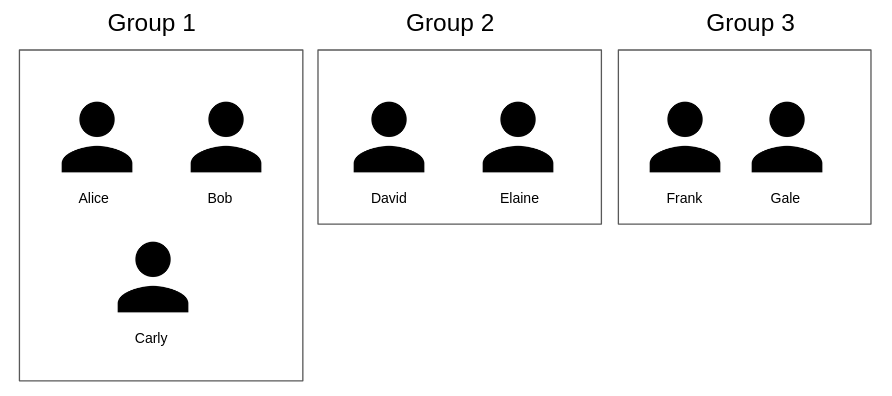
\includegraphics[width=10cm]{perm-comb-4.png}
\end{center}

\par\noindent [Alice, David,Frank],  [Alice, Elaine,Frank],
[Bob, David, Frank], [Bob, Elaine,Frank],
[Carly, David, Frank], [Carly, Elaine, Frank],
[Alice, David,Gale], [Alice, Elaine, Gale ],
[Bob, David, Gale ], [Bob, Elaine, Gale],
[Carly, David, Gale], [Carly, Elaine, Gale] 
\newline \newline
This is exactly what the rule predicts: (3)(2)(2) = 12
 \pagebreak
 \section {Counting Permutations}
 
 \par\noindent The number of permutations of a set is the number of possible arrangements (order matters). The number of permutations involving all elements of a set containing n elements is just:
 
 \begin{flalign}
 	P(n) = n!
 \end{flalign}
  

\par\noindent Suppose we have a group of people composed of Alice, Bob, Carly. All three  are office workers and upon clocking in can take any of the three  available cubicles in the office. We want to investigate how many possible arrangements of employee to cubicles are possible. 

\begin{center}
	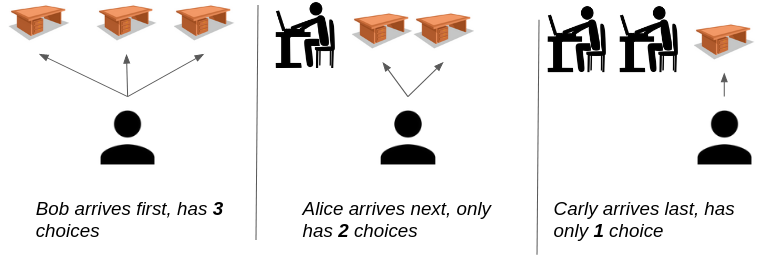
\includegraphics[width=10cm]{perm-comb-1.png}
\end{center}



\par\noindent The strategy to employ is as follows: if Alice takes the first cubicle, then Bob has one less to chose from, after Bob makes a selection Carly will have no choice but to take the one remaining cubicle. This results in 6 possible arrangements: 
\newline
\newline
[Alice, Bob, Carly] ,[Alice, Carly, Bob], [Bob, Alice, Carly], [Bob, Carly, Alice], [Carly, Alice, Bob], [ Carly, Bob, Alice]
\newline

\par\noindent This is consistent with the result of n!, int his case 3! = 6. 
\newline
\par\noindent One way to relate this idea back to the fundamental counting principle is by envisioning this exercise as counting the number of ways in which the cubicles might fill up. Suppose Bob arrived at the office first. He can pick from any of the cubicles, so he settles on one. Bob can pick from a set of 3. Now two things can happen, suppose Alice arrived next, Alice can therefore pick from a set of 2. Carly who arrives last can only pick from a set of 1. Therefore, Bob arriving first can lead to two possible arrangements. If we repeat this analysis with Bob arriving first, and then with Carly arriving first, we arrive at expected 6 arrangements.
\newline
\begin{center}
	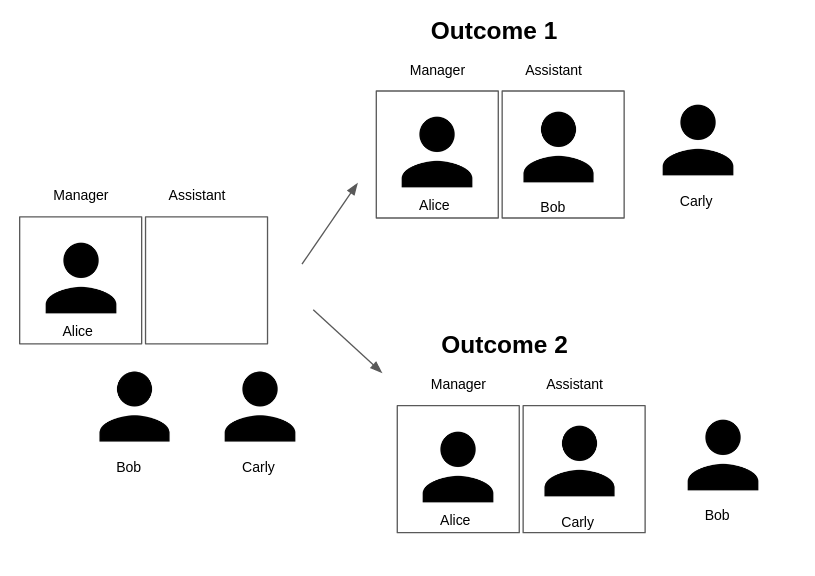
\includegraphics[width=8cm]{perm-comb-6.png}
\end{center}
\par\noindent The multiplicative nature of this line of thinking 3! = (3)(2)(1) is in fact just an application of the multiplication rule. 
\newline

\par\noindent We can also consider an arrangement of r elements within a set of n. The number of permutations in this case is: 

\begin{flalign}
	P(n,r) = \frac{n!}{(n-r)!}
\end{flalign}

\par\noindent Now suppose again that Alice, Bob, and Carly work at the same company. The company needs to chose one employee to be a project manager and another to be a project assistant. All three are qualified for either role. Using expression (1) we conclude that there are 6 possible arrangements: \( \frac{3!}{(3-2)!} \). With this small set, we can also arrive at this conclusion manually. If Alice is selected to be project manager, then two things can happen, either Bob is selected to be the assistant or Carly is selected. 

\begin{center}
	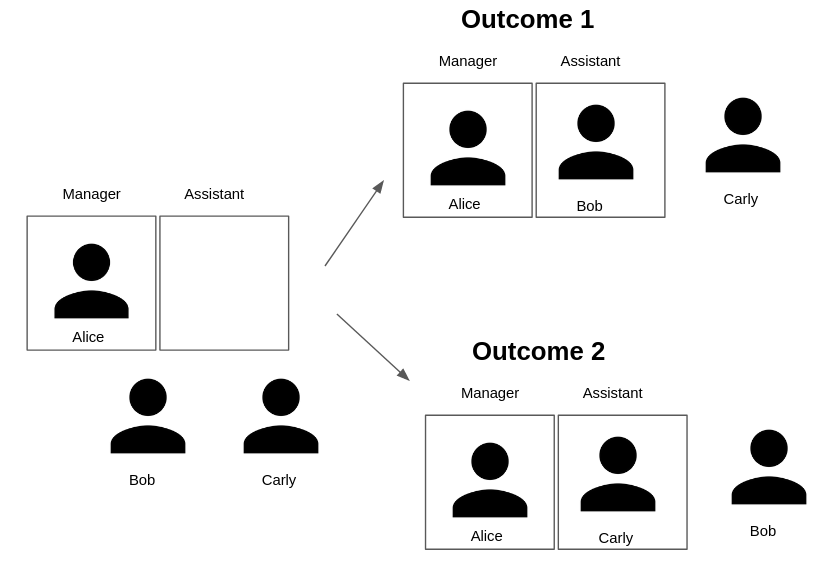
\includegraphics[width=10cm]{perm-comb-2.png}
\end{center}

\par\noindent If we repeat this analysis, we will find that if Bob gets selected to be the manager, then either Alice or Carly will be the assistant. A similar situation will ensue if Carly is selected to be the manager. Adding all the possible outcomes, we get 6.
\newline
\par\noindent We will now see how expression 2 is derived. In the previous example, we were calculating P(3,2). Let's pick some larger numbers, suppose we are calculating P(6,4). We can observe the following:

\begin{flalign*}
P(6,4) = \frac{6!}{(6-4)!} =  \frac{         (6)(5)(4)(3)(\cancel{2})(\cancel{1})}{(\cancel{2})(\cancel{1})}
\end{flalign*}

\par\noindent Seeing this simplification, we can restate expression (1) as the following product:

\begin{flalign*}
P(n,r) = (n)(n-1)(n-2) ... (n-r+1)
\end{flalign*}

\par\noindent We will multiply the expression above by\(\frac{(n-r)(n-r-1)...(3)(2)(1)}{(n-r)(n-r-1)...(3)(2)(1)}\) and perform a few cancellations.

\begin{flalign*}
P(n,r) = (n)(n-1)(n-2) ... (n-r+1) \frac{(n-r)(n-r-1)...(3)(2)(1)}{(n-r)(n-r-1)...(3)(2)(1)}
\end{flalign*}

\begin{flalign*}
P(n,r) = \frac{(n)(n-1)(n-2)...(n-r+1)(n-r)(n-r-1)...(3)(2)(1)}{(n-r)(n-r-1)...(3)(2)(1)}
\end{flalign*}

\begin{flalign*}
P(n,r) = \frac{n!}{(n-r)!}
\end{flalign*}

 \section {Counting Combinations}

\par\noindent If we count the possible arrangements without caring about order (i.e. Alice \& Bob is the same arrangement as Bob \& Alice) we have a combination. To find the combinations of length r from a set n we can use the formula:

\begin{flalign}
C(n,r)=\frac{n!}{r!(n-r)!}
\end{flalign}

\par\noindent Suppose that Alice, Bob, and Carly are again working for the same company. The company needs two volunteers for a task. All employees are equally qualified. How many pairings are possible? Again taking advantage of the small set size, we can work out that there are 3 pairings: Alice \& Bob, Alice \& Carly, and Bob \& Carly. This is consistent with the prediction from the combination formula: \(\frac{3!}{(2!)(3-2)!} \)

\begin{center}
	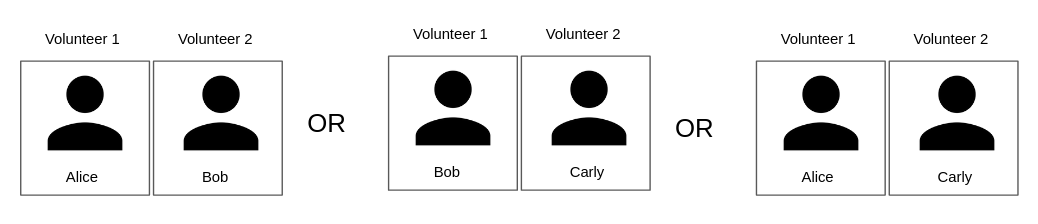
\includegraphics[width=10cm]{perm-comb-3.png}
\end{center}

\par\noindent Expression (2) can be rewritten in a more intuitive way:

\begin{flalign*}
	C(n,r)=\frac{n!}{(n-r)!} \; \; \frac{1}{r!}
\end{flalign*}

\par\noindent The expression now is basically just P(n,r), scaled by a factor of \(\frac{1}{r!}\). If a set has a length of r, then we know that the number of permutations is r!. Since order does not matter in combinations, we simply scale down P(n,r) by multiplying it with \(\frac{1}{r!}.\) 

\pagebreak
\section {Combinations And The Binomial Theorem}

\par\noindent The binomial thorem states that when performing an expansion, the coefficients can be calculated using expression(3). The formal definition is as follows:

 \begin{flalign*}
 	(x+y)^{n} = \sum_{r=0}^{n} C(n,r)x^{n-r}y^{r}
 \end{flalign*}

\par\noindent The cases for n=3, n=2, and n=1 are worked out below:

\begin{flalign*}
	(x+y)^{3} = C(3,0)x^{3}y^{0} + C(3,1)x^{2}y^{1} + C(3,2)x^{1}y^{2} + C(3,3)x^{0}y^{3} \\
	(x+y)^{3} = x^{3} + 3x^{2}y + 3xy^{2} + y^{3}	
\end{flalign*}

\begin{flalign*}
	(x+y)^{2} = C(2,0)x^{2}y^{0} + C(2,1)x^{1}y^{1} + C(2,2)x^{0}y^{2} \\
	(x+y)^{2} = x^{2} + 2xy + y^{2}
\end{flalign*}

\begin{flalign*}
	(x+y)^{1} = C(1,0)x^{1}y^{0} + C(1,1)x^{0}y^{1} \\
	(x+y)^{1} = x + y
\end{flalign*}

\par\noindent Let's look at the case  \((x+y)^{2}\) geometrically. Suppose we divided a square in a way that results in two sub-squares:

\begin{center}
	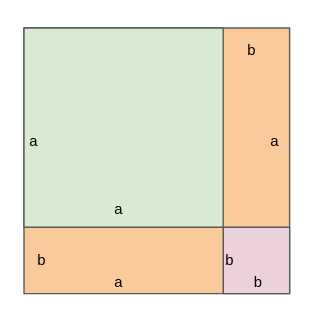
\includegraphics[width=7cm]{perm-comb-5.png}
\end{center}

\par\noindent The area of the two sub-squares are \(a^{2}\) and \(b^{2}\). We are also left with two rectangles each having an area of \(ab\). The sum of all the areas, \(a^{2} + ab + ab + b^{2} \), is in fact the binomial expansion of \((a+b)^{2}\). 
\newline
\par\noindent In this expansion, we know that the second term will be \(C(2,1)a^{1}b^{1}\) or \(2ab\). One intuitive interpretation of the second term is that there is no distinction (in terms of area) between the two rectangles with dimensions \(a \times b\). Picking one is as good as picking the other, so from these two identical rectangles, you can chose 1.

\end{document}

